\chapter{Het gebruik van Exceptions bij meerdere objecten.} \label{chap:Excep}

Bij deze opgave worden voor het eerst Exceptions toegepast. Deze worden vervolgens gebruikt in een multipliciteit situatie, bijvoorbeeld: 1 device heeft 0..5 leds.

\section{Exceptions} 
Bij het aanzetten van de Logled (de methode \texttt{void zetAan(string)}) kunnen meerdere soorten fouten optreden. Fouten zoals niet aangesloten, geen tijd meer, verkeerde kleur. Daarom is besloten om  exceptions te gaan toepassen. Dit wordt in Figuur \ref{fig:llExc} aangegeven.
\begin{figure}[h!]
	\captionsetup{justification=centering}
	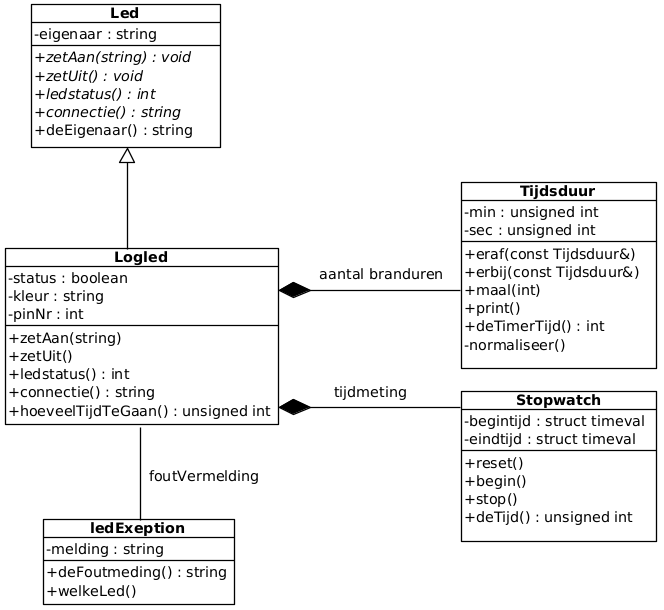
\includegraphics[width=0.9 \linewidth]{figuren/llExcept}     
\centering
\caption{De Logled die met exceptions kan gooien.}
\label{fig:llExc}
\end{figure} 
Hierbij wordt behalve de melding ook een verwijzing meegegeven naar de led waarbij de fout optreedt.
\newpage
\paragraph{Opdracht}

\begin{enumerate}
	\item Implementeer de klasse \textbf{LedException} (zowel de.h als de .cpp file).
	\item Pas de klasse Logled aan, zodat de exceptions gegenereerd kunnen worden.
	\item Wanneer de main van listing \ref{lst:logledEx} laat runnen,
wordt het volgende uitgeprint:\\
\texttt{Verkeerde kleur. De ledkleur is:groen Aangesloten op pin:132}
\begin{lstlisting}[caption=Twee objecten van de klasse \texttt{LogLed}. ,frame=trbl,firstnumber=1,numbers=left,label={lst:logledEx}]{Name}
	
int main()
{
	
	Logled logger(RODELEDPIN, "rood", "Pietje Puk", 0, 2);
	Logled sportled(GROENELEDPIN, "groen", "Bb", 0, 4);
	
	try
	{
		logger.zetAan("rood");
		sportled.zetAan("rood");
	}
	catch (LedException &le)
	{
		cout << le.deFoutmelding() << " Aangesloten op pin:" << le.welkeLed()->connectie() << endl;
	}
	usleep(DRIE_SEC);
	logger.zetUit();
	sportled.zetUit();
	
	return 0;
}
\end{lstlisting}		
\end{enumerate}
Laat het programma van Listing \ref{lst:logledEx} runnen, met hetzelfde resultaat.

\section{Toepassen van 1 op  0..5 multipliciteit.}
Het komt vaak voor dat het ene device verschillende diverse type leds kan bevatten. Zo kan de klasse DeviceLed van Figuur \ref{fig:devled} tot een maximum van 5 LEDs bevatten,   
\begin{figure}[h!]
	\captionsetup{justification=centering}
	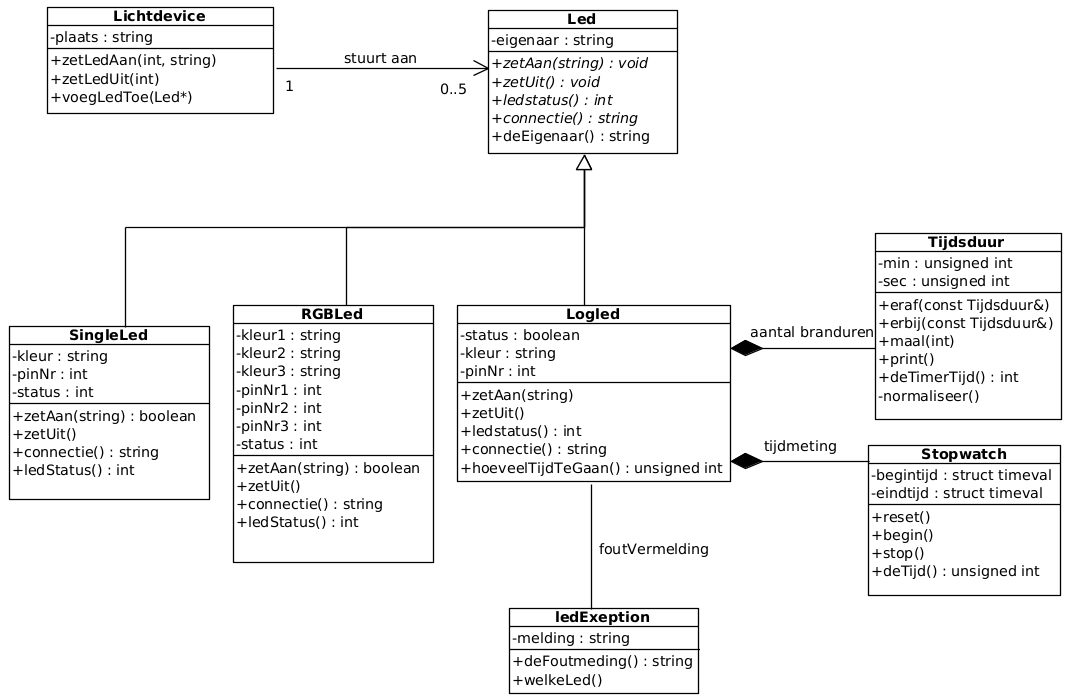
\includegraphics[width=1 \linewidth]{figuren/deviceled}     
	\centering
	\caption{Een device LED controleert meerdere leds.}
	\label{fig:devled}
\end{figure} 
die ieder afzonderlijk aangestuurd kan worden. 

\paragraph{Opdracht}

\begin{enumerate}
	\item Maak de klasse LedDevice. Houd hier wel rekening mee dat sommige leds met exceptions kunnen gooien. Indien dit zo is, stuur de ontvangen exception door.

\newpage
	\item Run het programma van listing \ref{lst:lichtdev}	

\begin{lstlisting}[caption=Twee objecten van de klasse \texttt{LogLed}. ,frame=trbl,firstnumber=1,numbers=left,label={lst:lichtdev}]{Name}
#include <iostream> // nodig voor cout (schrijven naar scherm)

int main() {
	Logled logger(RODELEDPIN,"rood","Pietje Puk",0,4);
	// Logled sportled(GROENELEDPIN,"groen","Bb",0,2);
	SingleLed sl1(GROENELEDPIN,"groen","L&B");
	RGBLed kl(RGB_R,RGB_G,RGB_B,"Pietje Puk");
	Lichtdevice lab1("D2.001");
	lab1.voegLedToe(&sl1);
	lab1.voegLedToe(&logger);
	lab1.voegLedToe(&kl);
	
	lab1.zetLedAan(0,"groen");
	usleep(TWEE_SEC);
	lab1.zetLedAan(2,"blauw");
	usleep(TWEE_SEC);
	lab1.zetLedAan(1,"rood");
	usleep(TWEE_SEC);
	for(int i=0;i<3;++i)
	lab1.zetLedUit(i);
}
\end{lstlisting}
	
	\item Pas listing  \ref{lst:lichtdev} aan, zodat een exception ontvangen kan worden en run deze.
	\item Start de VNC viewer op en run de DDD debugger en zet een breakpoint .
	\item Zet een breakpoint bij het statement: \textit{lab1.zetLedAan(1,"rood");} en display de Lichtdevice (lab1).
	 Als het goed is krijg je een afbeelding dat lijkt op Figuur \ref{fig:dddmld}
\begin{figure}[h!]
	\captionsetup{justification=centering}
	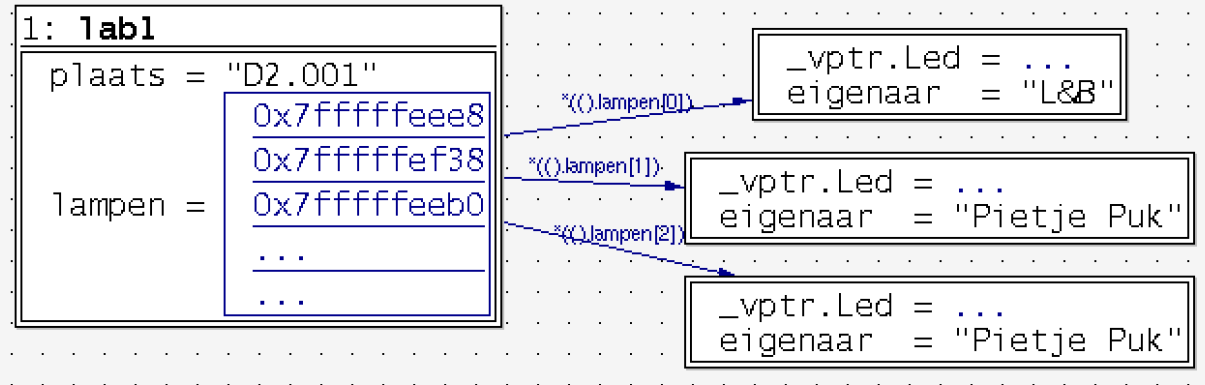
\includegraphics[width=0.95 \linewidth]{figuren/dddmeerdreld}     
	\centering
	\caption{Object Lichtdevice met 3 led objecten.}
	\label{fig:dddmld}
\end{figure}
Hierin is duidelijk te zien dat de verwijzingen(pointers) naar de base klasse \textbf{Led} zijn.
\item Print uit hoeveel tijd de logled (\texttt{logger}) nog heeft aan het einde van het programma.
\item Plaats het volgende in je portfolio:
\begin{itemize} 
\item De code van de klasse \textbf{Lichtdevice} (zowel de \texttt{.h} als de \texttt{.cpp} file).
\item De code van de  \texttt{int main();} functie waarbij de exceptions worden afgevangen.  
\item Je eigen afbeelding die lijkt op Figuur \ref{fig:dddmld}.
\item De code om de restant tijd van het object \texttt{logger} uit te printen. 
\end{itemize}	
	
\end{enumerate}